% ============================================================================
% ACADEMIC REVIEW PAPER TEMPLATE
% ============================================================================
% This template supports two citation styles:
%   - IEEE numbered (default):  \bibliographystyle{ieeetr}
%   - Author-year (natbib):    Uncomment the natbib block below and
%                              switch \bibliographystyle to {plainnat} or {abbrvnat}
%
% To switch to author-year:
%   1. Uncomment \usepackage{natbib} below
%   2. Change \bibliographystyle{ieeetr} → \bibliographystyle{plainnat}
%   3. Use \citep{key} / \citet{key} instead of \cite{key}
% ============================================================================

\documentclass[conference]{IEEEtran}
\IEEEoverridecommandlockouts

% ---------------------------------------------------------------------------
% CITATION STYLE CONFIGURATION
% ---------------------------------------------------------------------------
% For IEEE numbered citations (default), use:
\usepackage{cite}

% For author-year citations, uncomment this and comment \usepackage{cite} above:
% \usepackage[round]{natbib}
% \bibliographystyle{plainnat}    % author-year, ordered by author
% \bibliographystyle{abbrvnat}    % author-year, abbreviated first names
% \bibliographystyle{unsrtnat}    % author-year, ordered by appearance
% ---------------------------------------------------------------------------

% ---------------------------------------------------------------------------
% PACKAGES
% ---------------------------------------------------------------------------
\usepackage{enumitem}
\usepackage{amsmath,amssymb,amsfonts}

% Algorithms (common in CS/engineering)
\usepackage{algorithm}
\usepackage{algorithmic}

% Graphics
\usepackage{graphicx}
\usepackage{textcomp}
\usepackage{xcolor}
\usepackage{forest}        % Tree diagrams (useful for taxonomies across domains)
\usepackage{adjustbox}
\usepackage{url}

% TikZ — Used for: architecture diagrams (CS), pathway maps (biomed),
% reaction schemes (chemistry), schematic diagrams (physics), etc.
\usepackage{tikz}
\usetikzlibrary{
    shapes.geometric, arrows, positioning, fit, backgrounds,
    calc, decorations.pathreplacing, decorations.markings,
    patterns, circuits.logic.US, matrix, chains
}

% Plots — Used for: time series, dose-response curves, performance plots
\usepackage{pgfplots}

% Professional tables with publication-ready styling
\usepackage{booktabs}
\usepackage{colortbl}
\usepackage{threeparttable}
\usepackage{cuted}         % Multi-column environments

% Custom line-break in author block
\makeatletter
\newcommand{\linebreakand}{%
  \end{@IEEEauthorhalign}
  \hfill\mbox{}\par
  \mbox{}\hfill\begin{@IEEEauthorhalign}
}
\makeatother

% ---------------------------------------------------------------------------
% COLORS — Generic academic palette
% ---------------------------------------------------------------------------
\definecolor{primaryblue}{RGB}{55, 110, 180}
\definecolor{secondarygreen}{RGB}{50, 140, 80}
\definecolor{accentorange}{RGB}{230, 130, 30}
\definecolor{highlightred}{RGB}{190, 40, 50}
\definecolor{graytext}{RGB}{100, 100, 100}

% ---------------------------------------------------------------------------
% DOCUMENT BEGINS
% ---------------------------------------------------------------------------
\begin{document}

% ===========================================================================
% TITLE
% ===========================================================================
\title{[Paper Title — Specific and Descriptive]}

\author{
    \IEEEauthorblockN{
        [Author 1]\textsuperscript{*, a, b},
        [Author 2]\textsuperscript{a},
        [Author 3]\textsuperscript{c}
    }
    \IEEEauthorblockA{
        \textsuperscript{a}[Institution 1, Country]
    }
    \IEEEauthorblockA{
        \textsuperscript{b}[Institution 2, Country]
    }
    \IEEEauthorblockA{
        \textsuperscript{c}[Institution 3, Country]
    }
    \IEEEauthorblockA{
        *Corresponding Email: [email@example.com]
    }
}

\maketitle

% ===========================================================================
% KEYWORDS
% ===========================================================================
\begin{IEEEkeywords}
[Keyword 1], [Keyword 2], [Keyword 3], [Keyword 4], [Keyword 5]
\end{IEEEkeywords}

% ===========================================================================
% ABSTRACT (150–250 words)
% ===========================================================================
\begin{abstract}
[Summarize: (1) the research problem and its significance,
(2) the scope and methodology of this review,
(3) key findings or thematic synthesis,
(4) main conclusions and implications.
Be specific. Avoid citations in the abstract.]
\end{abstract}

% ===========================================================================
% 1. INTRODUCTION
% ===========================================================================
\section{Introduction}
[The introduction should:
\begin{itemize}
    \item Establish the importance and broader context of the topic
    \item State the problem or gap this review addresses
    \item Cite foundational and recent relevant work \cite{key1,key2}
    \item Define the review's scope (in-scope / out-of-scope)
    \item Outline contributions: what is novel about this review
    \item Provide a roadmap of the remaining sections
\end{itemize}

Example: Recent advances in [field] have enabled \cite{author2023survey}...]

% ===========================================================================
% 2. BACKGROUND / RELATED WORK
% ===========================================================================
\section{Background and Preliminaries}
[This section should:
\begin{itemize}
    \item Define core concepts, notation, and terminology (with citations)
    \item Provide historical context or a short timeline of key developments
    \item Distinguish this review from existing surveys \cite{smithmeta2022}
    \item Introduce the principal families of methods / theories at a high level
\end{itemize}

Use citations for all non-trivial claims: \cite{jones2024study}.]

\subsection{Core Definitions and Scope}
[Define key terms and assumptions used throughout the paper. Clarify what is
in-scope versus out-of-scope for this review.]

\subsection{Historical Development}
[Summarize the evolution of the field. A timeline or brief narrative with
landmark papers is often helpful.]

\subsection{Relation to Existing Reviews}
[Position this review relative to prior surveys or meta-analyses. State
explicitly what gap this review fills.]

% ===========================================================================
% 3. CORE APPROACHES / METHODS
% ===========================================================================
\section{Core Approaches and Methods}
[This is the central section of the review. Organize by approach family,
methodological category, or theoretical framework. For each approach:
\begin{itemize}
    \item Define the approach clearly (with equations if needed)
    \item Provide representative citations for each sub-category
    \item Discuss strengths, limitations, and typical use cases
    \item Compare and contrast with other approaches
\end{itemize}

If a taxonomy is useful, present it here with a figure or table.]

\subsection{Approach Category A}
[Describe the first major category of methods. Include representative examples
and key citations \cite{firstmethod2023}.]

\subsubsection{Key Variants}
[Discuss important variants within this category.]

\subsubsection{Strengths and Limitations}
[Evidence-based assessment of when this approach works well and when it fails.]

\subsection{Approach Category B}
[Second major category. Same structure as above.]

\subsection{Comparative Analysis}
[Cross-cutting comparison: a summary table is recommended here (see Table~\ref{tab:comparison}).]

% Example comparison table
\begin{table}[t]
\centering
\caption{Comparison of major approaches.}
\label{tab:comparison}
\begin{tabular}{lcccc}
\toprule
\textbf{Approach} & \textbf{Dimension 1} & \textbf{Dimension 2} & \textbf{Dimension 3} & \textbf{Key Refs} \\
\midrule
Category A \cite{a1} & High & Medium & Yes & \cite{a2,a3} \\
Category B \cite{b1} & Medium & High & Partial & \cite{b2,b3} \\
Category C \cite{c1} & Low & High & Yes & \cite{c2} \\
\bottomrule
\end{tabular}
\end{table}

% ===========================================================================
% 4. KEY CHALLENGES / OPEN PROBLEMS
% ===========================================================================
\section{Key Challenges and Open Problems}
[Identify and discuss the most significant unresolved issues in the field.
For each challenge:
\begin{itemize}
    \item Define the problem clearly, with evidence from the literature
    \item Cite recent attempts to address it (if any)
    \item Propose potential research directions
    \item Assess the difficulty and importance of the challenge
\end{itemize}

This section should be evidence-heavy and forward-looking.]

\subsection{Challenge 1: [Name]}
[Describe the challenge, its significance, and current status.]

\subsection{Challenge 2: [Name]}
[Same structure.]

% ===========================================================================
% 5. FUTURE DIRECTIONS
% ===========================================================================
\section{Future Directions}
[Synthesize promising research directions that emerge from the identified
challenges. Be specific — name concrete problems, not vague aspirations.
Ground each direction in the literature reviewed above.

This section can be combined with or placed before the Conclusion.]

% ===========================================================================
% 6. CONCLUSION
% ===========================================================================
\section{Conclusion}
[Summarize the review's main takeaways:
\begin{itemize}
    \item Restate the problem and scope (1 sentence)
    \item Summarize key patterns or themes identified (2–3 sentences)
    \item Highlight the most important open challenges (1 sentence)
    \item Conclude with a forward-looking statement
\end{itemize}

Do not introduce new claims or citations here.]

% ===========================================================================
% FIGURE EXAMPLES
% ===========================================================================
% Architecture / flowchart example
\begin{figure}[t]
    \centering
    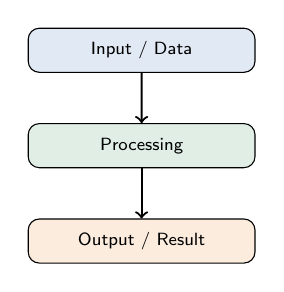
\begin{tikzpicture}[
        scale=0.8, transform shape,
        node distance=0.8cm,
        box/.style={
            rectangle, rounded corners, draw, fill=#1!15, text=black,
            minimum width=3.6cm, minimum height=0.7cm,
            align=center, font=\sffamily\footnotesize,
        },
    ]
        \node[box=primaryblue] (A) {Input / Data};
        \node[box=secondarygreen, below=of A] (B) {Processing};
        \node[box=accentorange, below=of B] (C) {Output / Result};

        \draw[->, thick] (A) -- (B);
        \draw[->, thick] (B) -- (C);
    \end{tikzpicture}
    \caption{[Descriptive caption. The figure should be self-contained.]}
    \label{fig:example}
\end{figure}

% ===========================================================================
% BIBLIOGRAPHY
% ===========================================================================
% For IEEE numbered citations (default with \usepackage{cite}):
\bibliographystyle{ieeetr}

% For author-year (uncomment when using natbib):
% \bibliographystyle{plainnat}

\bibliography{ref}

\end{document}
